% !TEX root = main.tex
\documentclass[11pt,xcolor={dvipsnames},hyperref={pdftex,pdfpagemode=UseNone,hidelinks,pdfdisplaydoctitle=true},usepdftitle=false]{beamer}
\usepackage{../include/presentation}
\usepackage{tikz}
\title{Multi-Robot Waypoint Inspection Plan Mixed Integer Linear Programming Project}
\author{Juan Carlos Cruz - ira406}
\date{ME 6033 Linear and Mixed Integer Optimization}
\begin{document}
    
    \begin{frame}
      \titlepage
      April 2025
    \end{frame}
    
    \begin{frame}{Introduction}
      \begin{itemize}
        \item Motivated by outdoor construction site inspection challenges
        \item Precast concrete elements require efficient inspection methods
        \item Multi-robot approach:
          \begin{itemize}
            \item Aerial robots locate targets
            \item Ground robots perform detailed inspections
          \end{itemize}
        \item Need for flexible inspection plans in dynamic environments
        \item MILP approach maximizes inspection coverage
      \end{itemize}
    \end{frame}

    \begin{frame}{Problem Description}
      \begin{itemize}
        \item Two robot types: aerial and ground mobile robots
        \item Inspection targets as waypoints in a 2D plane
        \item Sequential operation:
          \begin{itemize}
            \item Aerial robots verify waypoint location first
            \item Ground robots perform detailed inspection second
          \end{itemize}
        \item Robot constraints:
          \begin{itemize}
            \item Fixed speeds (meters/minute)
            \item Limited operation time (battery endurance)
            \item Required inspection time at waypoints
          \end{itemize}
        \item Objective: Maximize waypoint visits in a single inspection loop
      \end{itemize}
    \end{frame}

    \begin{frame}{Literature Review}
      \begin{itemize}
        \item Problem resembles multiple traveling salesman problem (mTSP)
        \item Prior works demonstrate multi-robot planning applications
        \item Traditional MILP for mTSP:
          \begin{itemize}
            \item Routing variables 
            \item Subtour elimination constraints
          \end{itemize}
        \item Simplification: Route length approximation
        \item Roundtrip distances from depot to waypoints estimate travel times
      \end{itemize}
    \end{frame}

    \begin{frame}{Model}
      \begin{columns}
        \begin{column}{0.5\textwidth}
          \textbf{Sets \& Parameters:}
          \begin{itemize}
            \item Waypoints $N$, indexed by $i$
            \item Aerial robots $K$, ground robots $L$
            \item Speeds: $s_A$, $s_G$
            \item Max operation times: $T_A^{max}$, $T_G^{max}$
            \item Inspection times: $t_A^{insp}$, $t_G^{insp}$
          \end{itemize}
        \end{column}
        \begin{column}{0.5\textwidth}
          \textbf{Decision Variables:}
          \begin{itemize}
            \item $w_i^{a,k}$: Aerial robot $k$ visits waypoint $i$
            \item $w_i^{g,l}$: Ground robot $l$ visits waypoint $i$
            \item $a_i^k$: Aerial completion time
            \item $g_i^l$: Ground completion time
            \item $use_k^a$, $use_l^g$: Robot usage
          \end{itemize}
        \end{column}
      \end{columns}
      \vspace{0.5cm}
      \textbf{Objective:} Maximize $\sum_{i \in N}\sum_{l \in L} w_i^{g,l}$
      \vspace{0.3cm}
      
      \textbf{Key Constraints:}
      \begin{itemize}
        \item Assignment: One robot per waypoint 
        \item Precedence: Aerial robots visit before ground robots
        \item Time constraints: Inspection durations, battery limits
      \end{itemize}
    \end{frame}

    \begin{frame}{Solution Method}
      \begin{itemize}
        \item Implemented in Python using PuLP library
        \item CBC solver from PuLP used for optimization
        \item Interactive browser-based GUI developed:
          \begin{itemize}
            \item Parameter input for robot specifications
            \item Waypoint location setting
            \item Real-time solution visualization
          \end{itemize}
        \item Code available at GitHub repository
      \end{itemize}
      
      % Insert demo image
      \begin{figure}
        \centering
        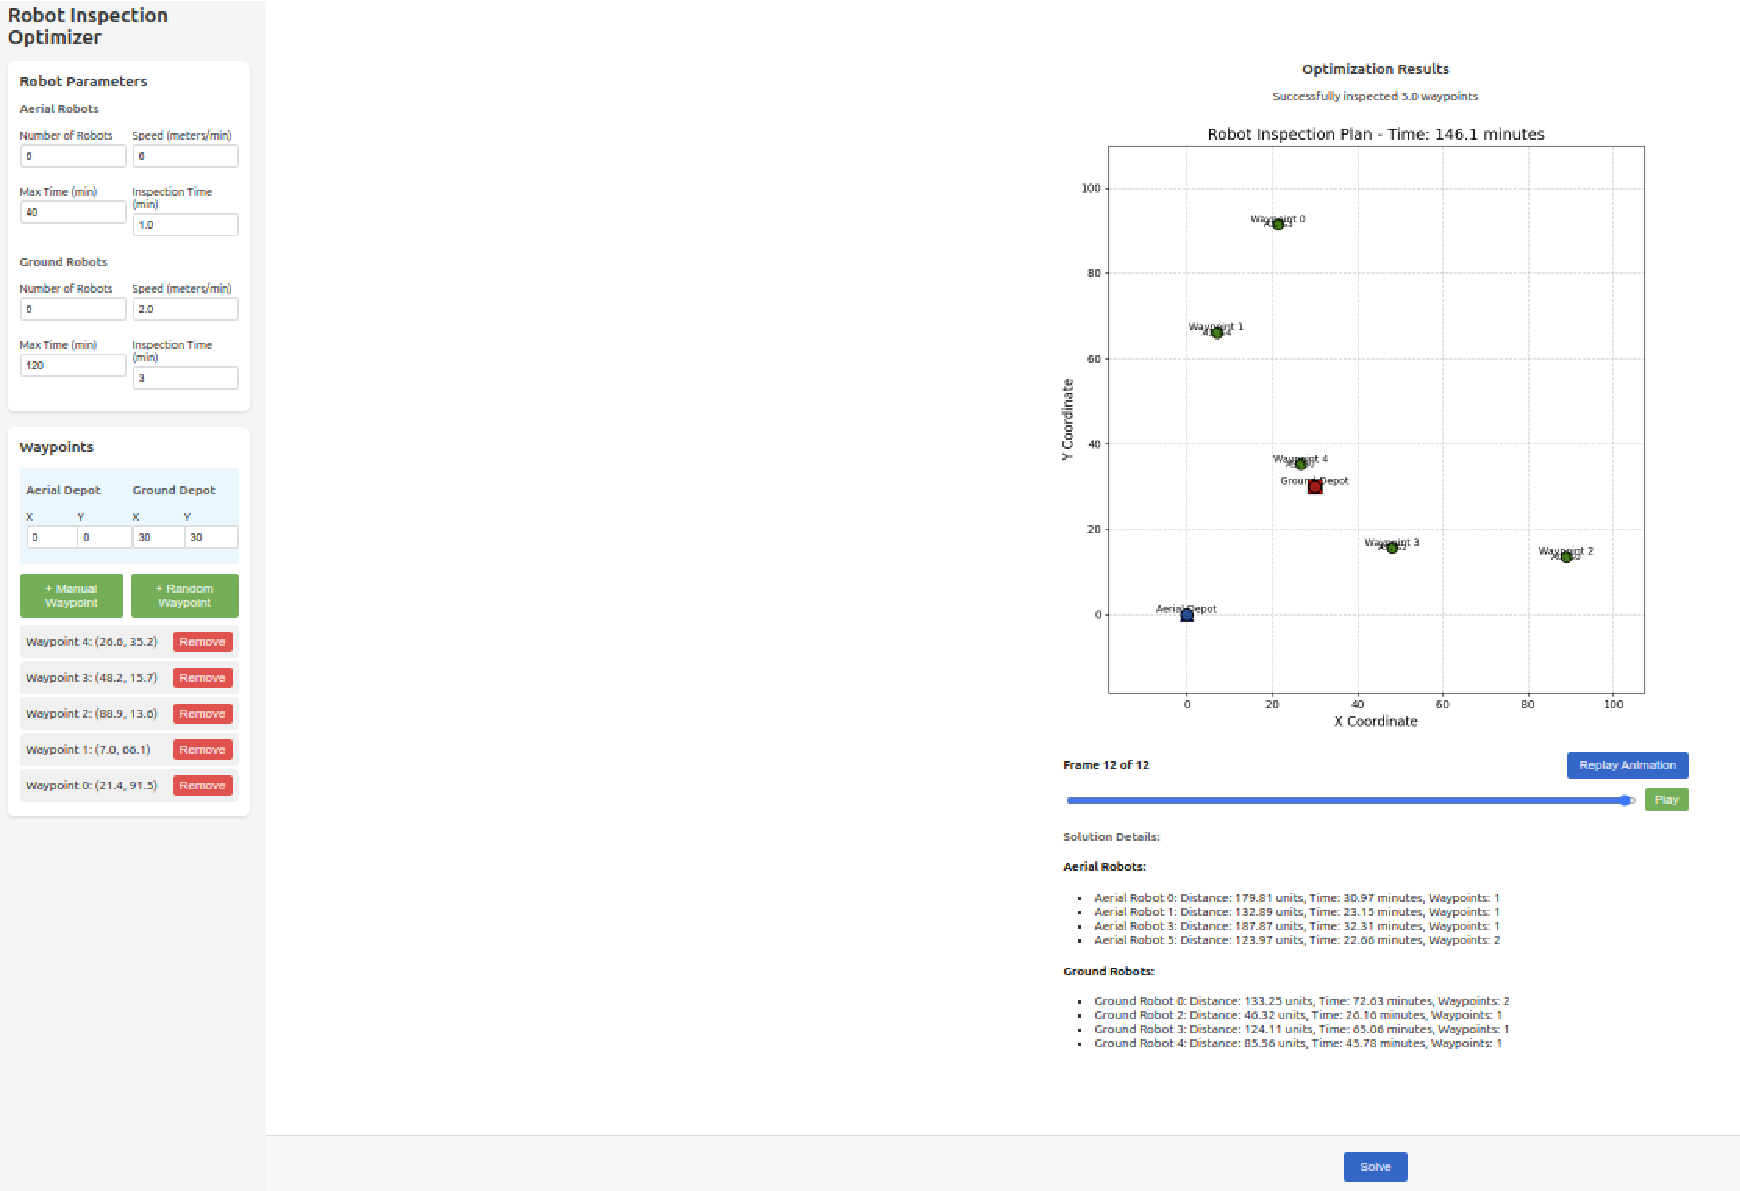
\includegraphics[width=0.7\linewidth]{figures/insp.pdf}
        \caption{Browser-based GUI showcasing solved inspection plan}
      \end{figure}
    \end{frame}

    \begin{frame}{Numerical Results - Computational Performance}
      \begin{itemize}
        \item Testing environment: 
          \begin{itemize}
            \item Intel i7, Python 3.12 Docker container
            \item 500s solver time limit
          \end{itemize}
        \item Non-monotonic scaling behavior:
          \begin{itemize}
            \item Solution time peaks at 15 waypoints then decreases
            \item Computation time peaks at 500m map size
          \end{itemize}
      \end{itemize}
      
      % Insert performance figures
      \begin{figure}
        \centering
        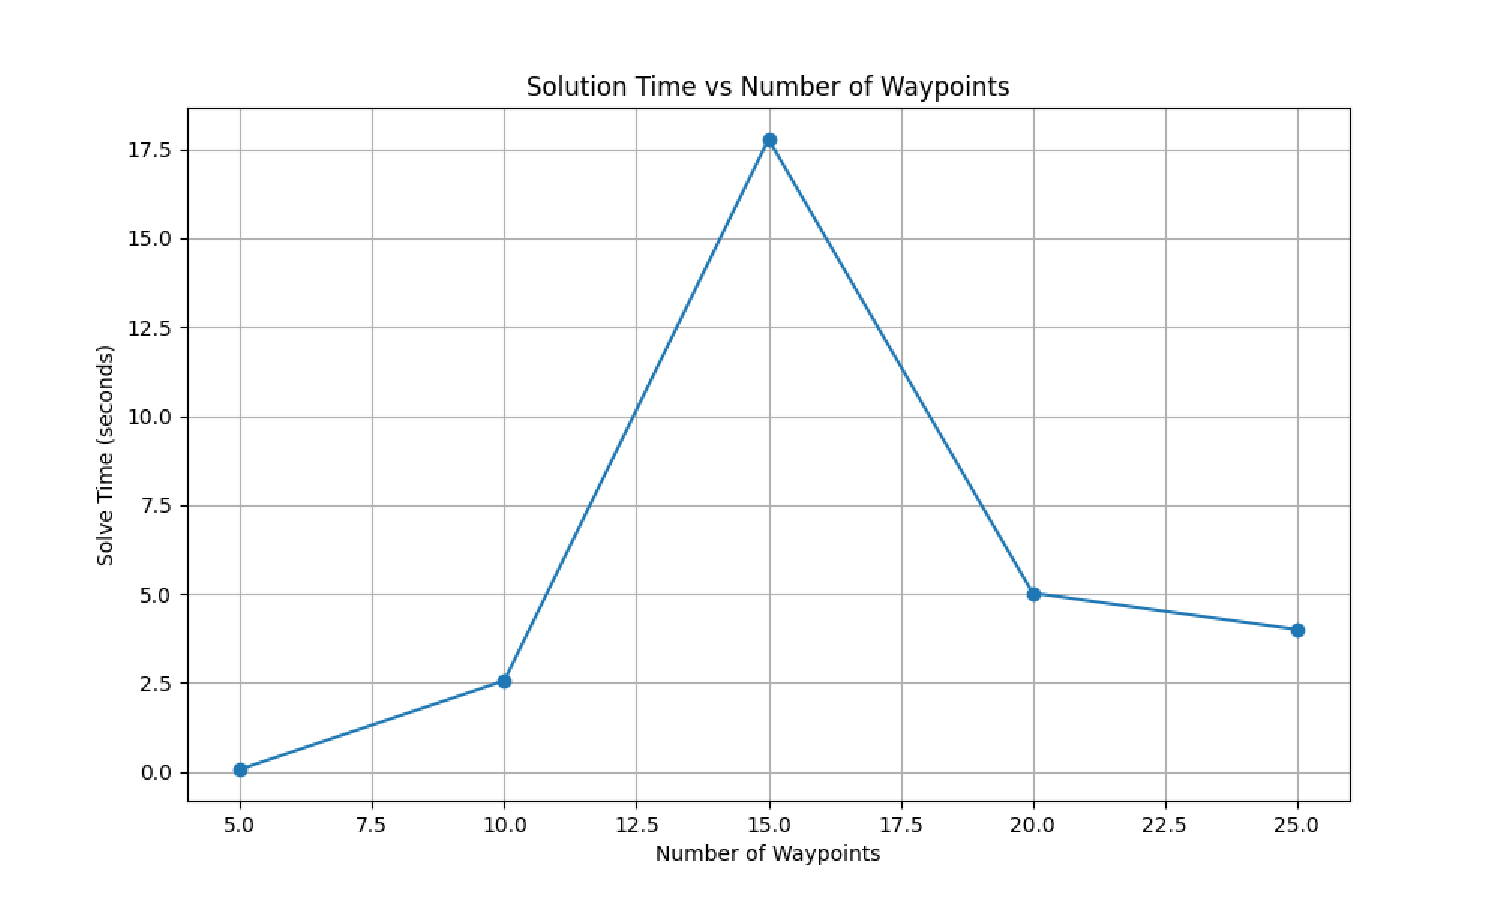
\includegraphics[width=0.48\linewidth]{figures/waypoints_vs_time.pdf}
        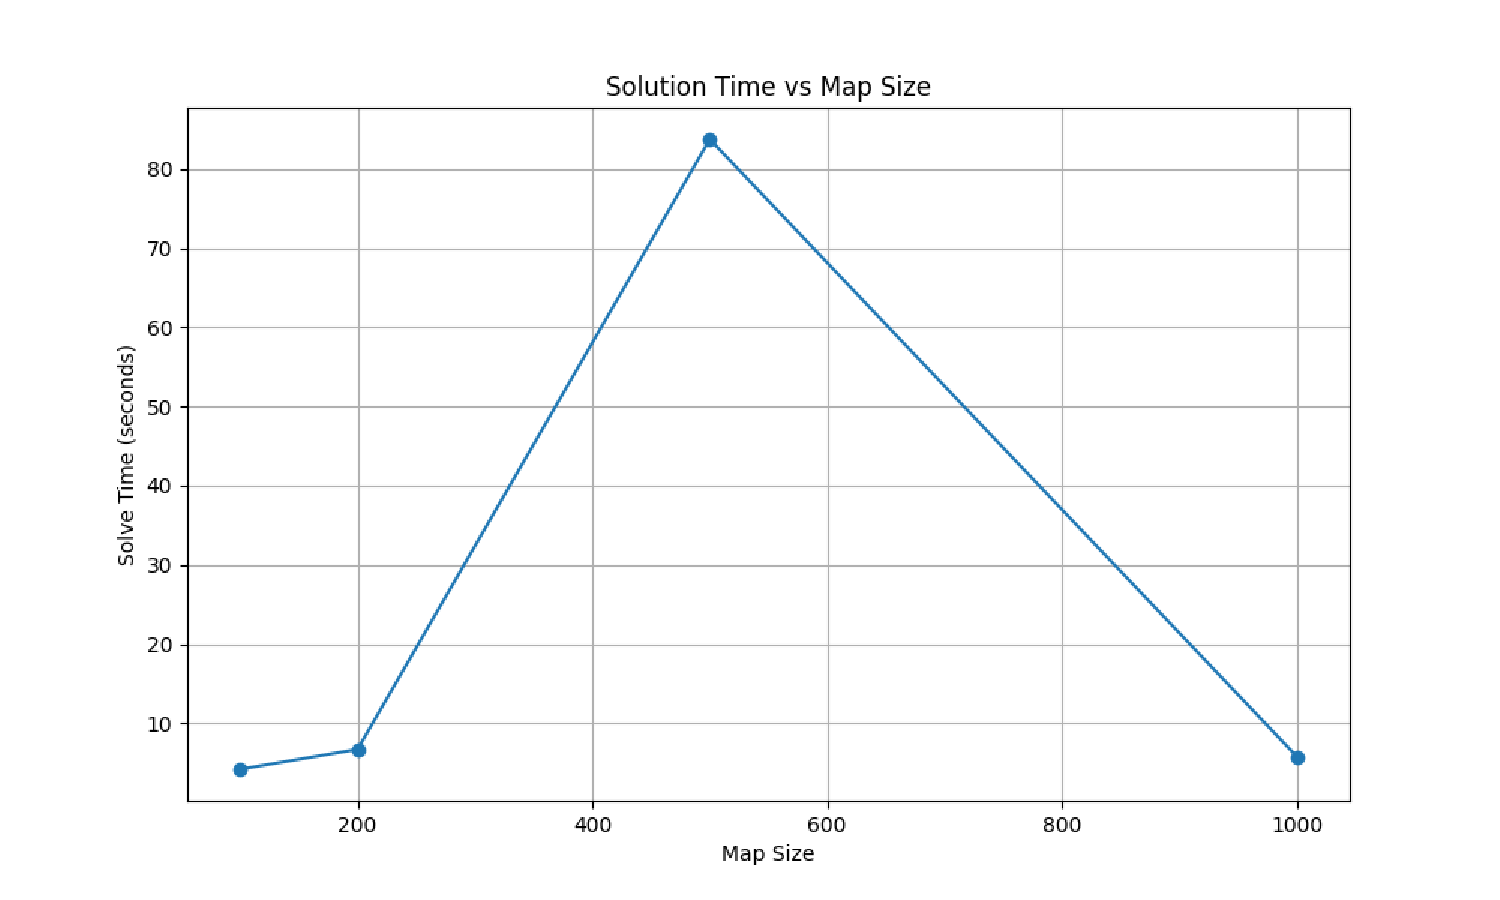
\includegraphics[width=0.48\linewidth]{figures/map_size_vs_time.pdf}
        \caption{Left: Solution time vs waypoint count. Right: Solution time vs map size}
      \end{figure}
    \end{frame}

    \begin{frame}{Numerical Results - Sensitivity Analysis}
      \begin{itemize}
        \item Most influential parameters:
          \begin{itemize}
            \item Number of ground robots
            \item Aerial robot maximum operation time
          \end{itemize}
        \item Significant impact: Robot speeds
        \item Minimal impact: Inspection times
      \end{itemize}
      
      % Insert tornado chart
      \begin{figure}
        \centering
        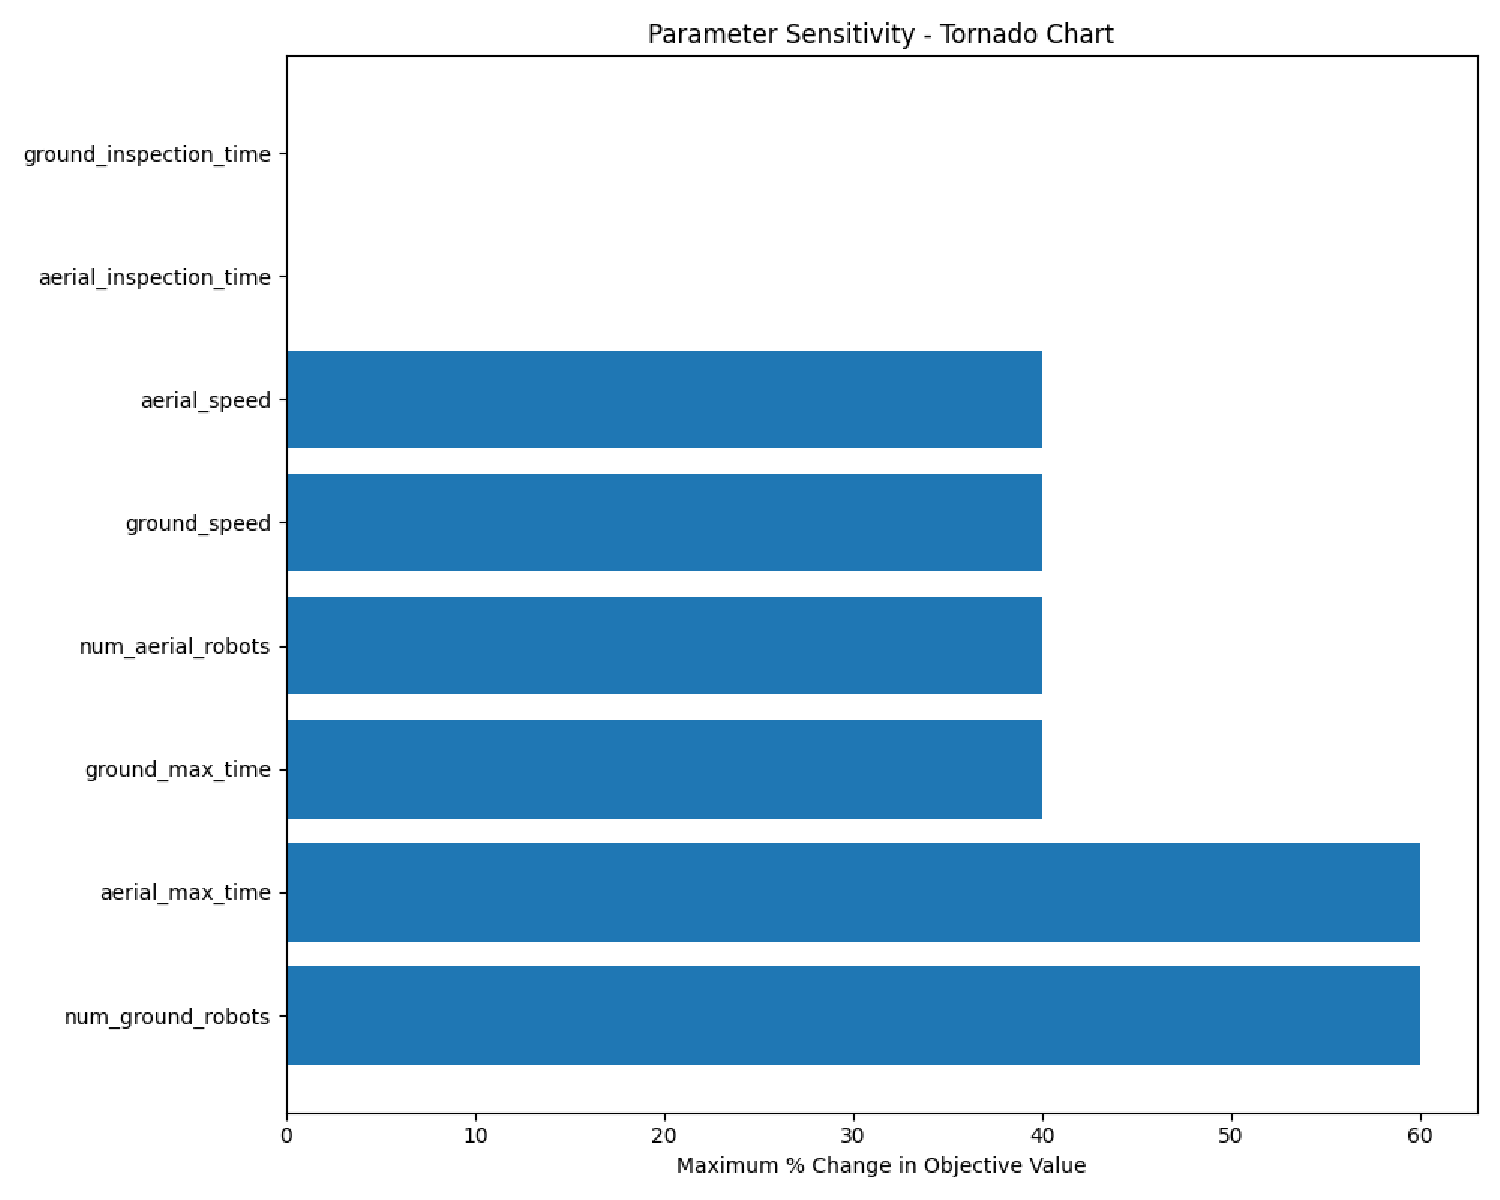
\includegraphics[width=0.5\linewidth]{figures/tornado_chart.pdf}
      \end{figure}
    \end{frame}

    \begin{frame}{Demo Video}
      \centering
      
    \end{frame}
    
    \lastslide
\end{document}